%This work is licensed under the Creative Commons
%Attribution-ShareAlike 4.0 International License. To view a copy of
%this license, visit http://creativecommons.org/licenses/by-sa/4.0/ or
%send a letter to Creative Commons, PO Box 1866, Mountain View, CA
%94042, USA.

%compile with: "pdflatex --shell-escape lesson_5.tex"

%This work is licensed under the Creative Commons
%Attribution-ShareAlike 4.0 International License. To view a copy of
%this license, visit http://creativecommons.org/licenses/by-sa/4.0/ or
%send a letter to Creative Commons, PO Box 1866, Mountain View, CA
%94042, USA.

%\documentclass[gray,handout, pdftex, 11pt]{beamer}
%\documentclass[handout, pdftex, 11pt]{beamer}

\documentclass[pdftex, 11pt]{beamer}

\usepackage[utf8]{inputenc}
\usepackage[T1]{fontenc}
\usepackage{lmodern}
%\usepackage[italian]{babel}
\usepackage{graphicx}
\usepackage{listings}
\usepackage{microtype}
\usepackage{acronym}
\usepackage{array}
\usepackage{tikz}
\usetikzlibrary{shapes, chains, scopes, shadows, positioning, arrows,
  decorations.pathmorphing, calc}

\colorlet{c1}{green!20}
\colorlet{c2}{blue!10}
\colorlet{drawColor}{black!50}
\colorlet{commentColor}{green!70!black!90}

\tikzstyle{oval}=[ellipse, align=center, drop shadow, draw=drawColor, fill=white]
\tikzstyle{rect}=[rectangle, rounded corners=2pt, align=center, drop
shadow, draw=drawColor, fill=white]
\tikzstyle{comment}=[text=commentColor,font=\itshape]
\tikzstyle{textLab}=[]
\tikzstyle{arrow}=[->, very thick, >=stealth', draw=black!80]
\tikzstyle{darrow}=[->, dash pattern=on 3pt off2pt, very thick, >=stealth', draw=black!80]
\tikzstyle{fStartEnd}=[ellipse, align=center, drop shadow, draw=drawColor, fill=white]
\tikzstyle{fInput}=[trapezium, trapezium left angle=70, trapezium right angle=110,
align=center, drop shadow, draw=drawColor, fill=white]
\tikzstyle{fProcess}=[rectangle, align=center, drop shadow, draw=drawColor, fill=white]
\tikzstyle{fSelection}=[diamond, shape aspect=3, align=center, drop
shadow, draw=drawColor, fill=white]
\tikzstyle{fOutput}=[tape, tape bend top=none, align=center, drop shadow, draw=drawColor, fill=white]
\tikzstyle{mem}=[rectangle, align=center, draw=drawColor, fill=white]
\tikzstyle{clo}=[cloud, aspect=2, align=center, drop shadow, draw=drawColor, fill=white]

\lstdefinestyle{customc}{
   language=C,
   % basicstyle=\small\ttfamily\bfseries,
   basicstyle=\ttfamily,
   keywordstyle=\color{blue}\ttfamily,
   stringstyle=\color{red}\ttfamily,
   commentstyle=\color{green}\ttfamily,
   morecomment=[l][\color{magenta}]{\#},
   % breaklines=false,
    breaklines=true, breakatwhitespace=false,
   frameround=fttt,
   frame=trBL,
   backgroundcolor=\color{yellow!20},
   numbers=left,
   stepnumber=1,    
   firstnumber=1,
   numberfirstline=true,
   numberstyle=\tiny\color{black!50},
   xleftmargin=2em,
   framexleftmargin=1.5em
   % linewidth=8cm,
}

\lstnewenvironment{cblock}[1][]
{
  \lstset{
    style=customc,
    #1
  }
}{}

\newcommand{\cfile}[2][]{
  \lstinputlisting[style=customc, #1]{#2}
}

\definecolor{links}{HTML}{2A1B81}
\hypersetup{colorlinks,linkcolor=links,urlcolor=links}

\definecolor{links}{HTML}{2A1B81}
\hypersetup{colorlinks,linkcolor=,urlcolor=links}


\mode<presentation>{
  %-------------------------1
  \usetheme{Boadilla}
  \usecolortheme{beaver}
  %-------------------------1
  %-------------------------2
  %\usetheme{Goettingen}
  %\usecolortheme{sidebartab}
  %-------------------------2
  %\useoutertheme[right]{sidebar}
  %\usefonttheme{default}
  \setbeamercovered{transparent}
  %\setbeameroption{show notes on second screen=right}
  \setbeamertemplate{navigation symbols}{}
  \setbeamertemplate{footline}{}

  \bibliographystyle{abbrv}  
  %\renewcommand\bibfont{\scriptsize}
  \setbeamertemplate{bibliography item}{\textbullet}
  \setbeamertemplate{itemize item}{\checkmark}
  \setbeamertemplate{itemize subitem}{-}
  \setbeamertemplate{enumerate items}[default]
  \setbeamertemplate{sections/subsections in toc}[square]
}

\subtitle{Logical Computational Thinking}
\institute[Tecnológico de Monterrey]{
  
\includegraphics[width=5cm]{img/logoTEC.jpg}\\[5mm]
  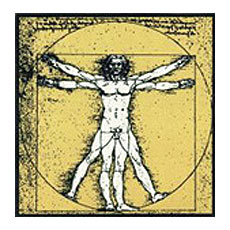
\includegraphics[width=1cm]{img/logoLEO.jpg}
  Scuola Leonardo Da Vinci (Firenze)
}

\author[Stefano Martina]{
  %\\[0.2cm]
  \textbf{Stefano MARTINA}\\
  {\small stefano.martina@gmail.com}
}

\titlegraphic{\tiny
  \href{http://creativecommons.org/licenses/by-sa/4.0/}{
\includegraphics[width=1cm]{img/logoCC.png}}
  This work is licensed under a
  \href{http://creativecommons.org/licenses/by-sa/4.0/}{Creative
    Commons Attribution-ShareAlike 4.0 International License}.}


\title[Lesson 5]{\textbf{Lesson 5 - Exercise}}
\date[21/9/15]{\flushright 21 September 2015}

\begin{document}

\begin{frame}[plain]
  \titlepage
\end{frame}

\begin{frame}
  \frametitle{Problem}
  \begin{block}{Background}
    \footnotesize
    You work for the \emph{New Horizons} mission. Few months ago the
    probe flew near \emph{Pluto}, but it is still in the \emph{Kuiper
      belt} and the mission is not yet concluded.

    The astrophysicists
    wants you to build a program for calculating when the probe will
    reach the end of the belt, or more in general when it  will reach
    a certain distance from the sun.
  \end{block}
  \begin{center}
    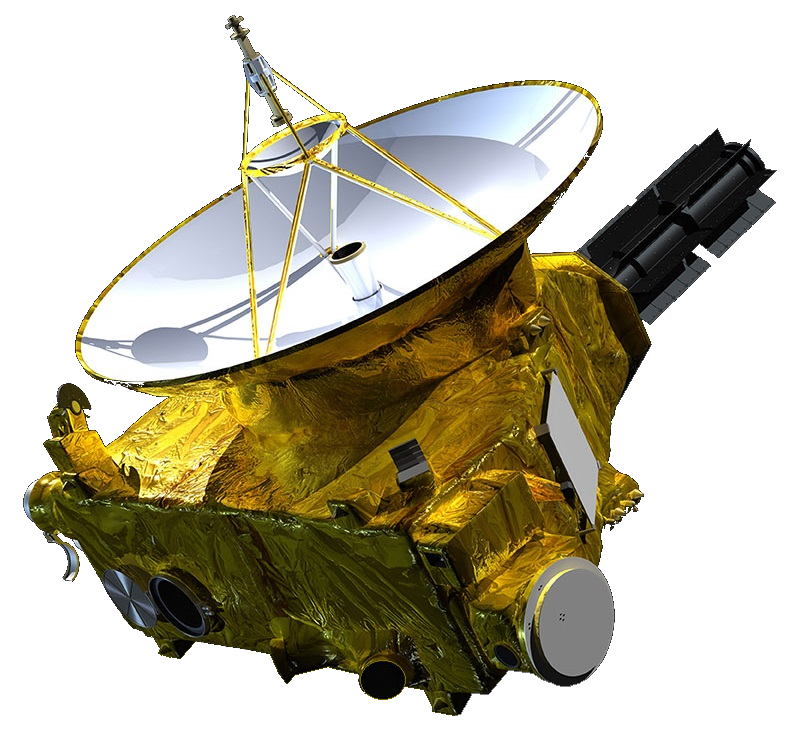
\includegraphics[width=0.45\textwidth]{img/New_Horizons.png}
    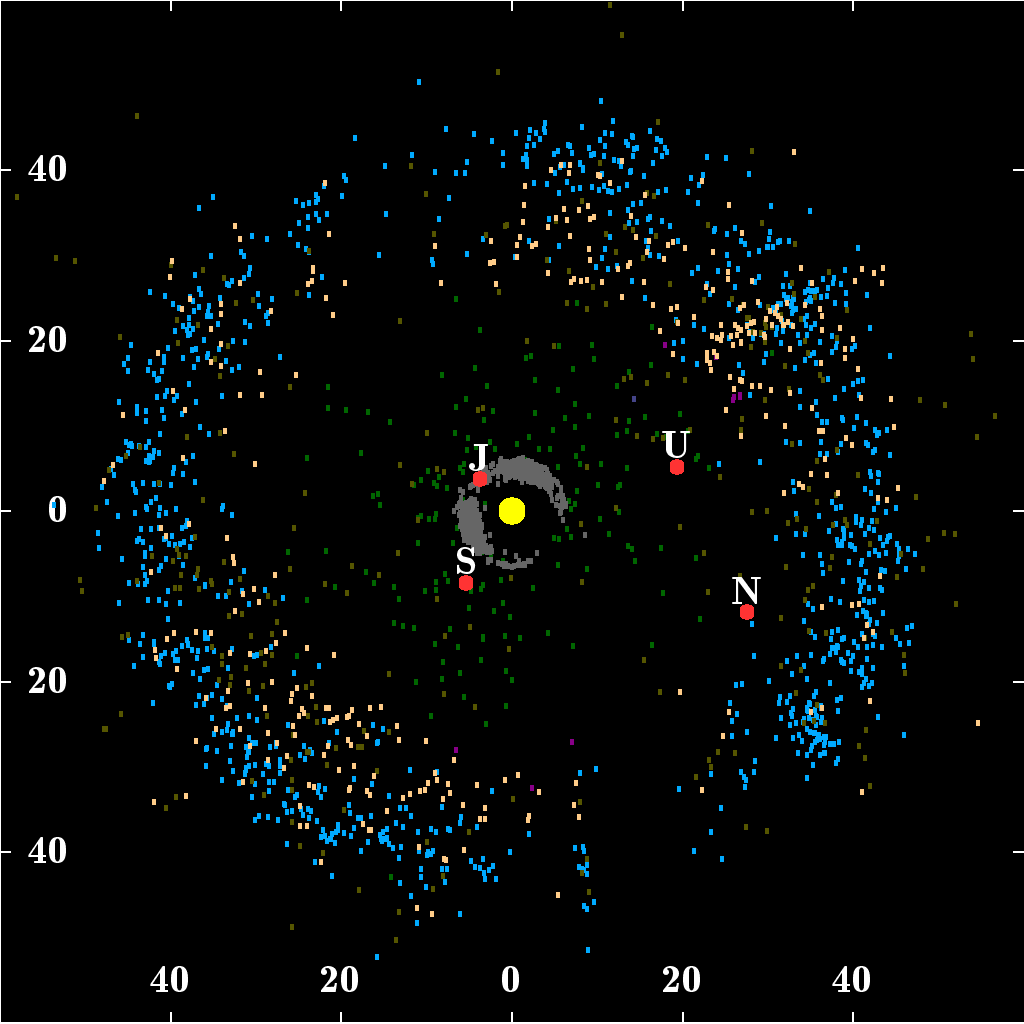
\includegraphics[width=0.45\textwidth]{img/Kuiper_belt.png}    
  \end{center}
\end{frame}

\begin{frame}
  \immediate\write18{wget -O img/whereIs_NewHorizons.svg http://pluto.jhuapl.edu/whereisnh/overview/nhov20150901_0445.svg}
  \immediate\write18{inkscape -f img/whereIs_NewHorizons.svg -A img/whereIs_NewHorizons.pdf}
  \begin{columns}[T]
    \begin{column}{0.65\textwidth}
      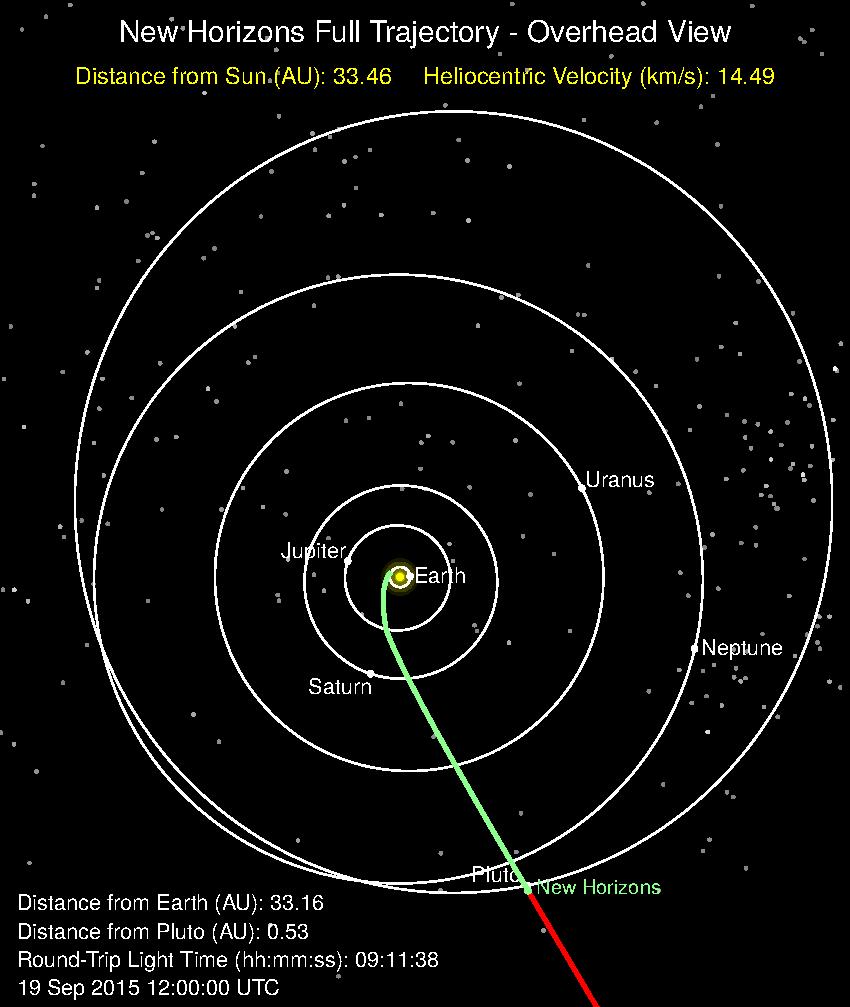
\includegraphics[width=\textwidth]{img/whereIs_NewHorizons.pdf}
    \end{column}
    \begin{column}{0.35\textwidth}
      \begin{block}{Astronomical Units (AU)}
        $1\ AU$ is approximately the average distance
        from the Sun to Earth, and the exact value is:
        \footnotesize
        \begin{eqnarray*}
        1\ AU &=& 149597870700\ m\\
        &=& 149597870,700\ km          
        \end{eqnarray*}
        \normalsize
      \end{block}
      \begin{itemize}
        \footnotesize
      \item \url{http://pluto.jhuapl.edu/}
      \item \url{https://www.nasa.gov/mission_pages/newhorizons/main/index.html}
      \item \url{https://it.wikipedia.org/wiki/New_Horizons}
      \item \url{https://en.wikipedia.org/wiki/Kuiper_belt}
      \end{itemize}
    \end{column}
  \end{columns}
\end{frame}

\begin{frame}
  \frametitle{Model}
  \begin{block}{Input}
    \begin{itemize}
    \item Current \alert{distance} from the Sun (in AU)
    \item Current \alert{velocity} respect the Sun in radial direction (in km/sec)
    \item \alert{Target} distance from the Sun (in AU)
    \end{itemize}
  \end{block}
  \begin{block}{Output}
    \begin{itemize}
    \item The necessary \alert{time} from now to reach the target (in sec)
    \end{itemize}
  \end{block}
  \begin{block}{Approximations}
    \begin{itemize}
    \item New Horizons probe is not going in radial direction respect
      the sun, but for
      now we can assume a radial direction and ignore the error
      \begin{itemize}
      \item An improvement to the program can be the possibility to
        specify the angular deviation from the radial direction
      \end{itemize}
    \end{itemize}
  \end{block}
\end{frame}

\begin{frame}
  \begin{block}{Physics}
    After the acceleration phases (\url{https://en.wikipedia.org/wiki/Gravity_assist}), probes are moving in \alert{uniform linear
    motion}, the law that govern it is:
    \begin{equation*}
      \Delta x = v \cdot \Delta t
    \end{equation*}
    where \alert{$\Delta x$} is the distance covered in \alert{$\Delta t$} time by a
    body that is moving at a constant velocity \alert{$v$} in a
    linear direction.
  \end{block}
  So if you know the position $x_p$ and the velocity $v_p$ of the
  probe, and the position $x_t$ of the target in the radial
  rectilinear direction you can calculate:
  \begin{eqnarray*}
    \Delta x&=&x_t - x_p\\
    \Delta t&=&\frac{\Delta x}{v_p}=\frac{x_t - x_p}{v_p}
  \end{eqnarray*}
\end{frame}

\begin{frame}
  \begin{block}{Unit of measures}
    For doing the calculations you need coherent unit of measures, so
    if $x_p$ and $x_t$ are expressed in $AU$ and $v_p$ is in $km/s$,
    first is necessary to convert $x_p$ and $x_t$ in $km$ using:
    \begin{eqnarray*}
      1\ AU&=&149\:597\:870\:700\ m\\
      &=&149\:597\:870,700\ km          
    \end{eqnarray*}
  \end{block}
\end{frame}

\begin{frame}
  \frametitle{Algorithm}
  \begin{center}
    \begin{tikzpicture}[node distance=5mm, font=\footnotesize, auto]
      \node(start) [fStartEnd] {Start};

      \node(input) [fInput, below=of start] {position, velocity, target};
      \draw [arrow] (start) -- (input);

      \node(selection) [fSelection, below=of input, shape aspect=1] {target\\$>$\\
        position?};
      \draw [arrow] (input) -- (selection);

      \node(int1a) [fInt, below=of selection] {1};
      \draw [arrow] (selection) -- node [near start] {yes} (int1a);

      \node(int2a) [fInt, right=20mm of int1a] {2};
      \draw [arrow] (selection) -| node [near start] {no} (int2a);

      \node(int1b) [fInt, right=50mm of start] {1};
      \node(int2b) [fInt, right=25mm of int1b] {2};

      \node(convert1) [fProcess, below=of int1b] {convert position in km};
      \draw [arrow] (int1b) -- (convert1);

      \node(convert2) [fProcess, below=of convert1] {convert target in km};
      \draw [arrow] (convert1) -- (convert2);

      \node(calcDistance) [fProcess, below=of convert2]
      {distance = target - position};
      \draw [arrow] (convert2) -- (calcDistance);
   
      \node(calcTime) [fProcess, below=of calcDistance]
      {time = distance / velocity};
      \draw [arrow] (calcDistance) -- (calcTime);
     
      \node(output) [fOutput, below=of calcTime] {time};
      \draw [arrow] (calcTime) -- (output);
 
      \node(outputErr) [fOutput, below=15mm of int2b] {ERROR\\(surpassed)};
      \draw [arrow] (int2b) -- (outputErr);

      \node(end) [fStartEnd, below=of output] {End};
      \draw [arrow] (output) -- (end);
      \draw [arrow] (outputErr) |- ($ (end.north) + (0,2mm) $);
    \end{tikzpicture}
  \end{center}
\end{frame}
\end{document}
